\documentclass[main.tex]{subfiles}
\begin{document}
\section{Introduction}

\subsection{Dead Reckoning}
% explain the issues of dead Reckoning
% use as an introduction: 
% 	to the FWKin prob.
% 	to the different sensors used

%todo: fix 1st sent.

Robot localization is crucial to effective robot locomotion. Various methods are
used to determine the current and future locations of robot; each unique to the
available sensors, robot structure and environment. Dead reckoning is one of the
simpler methods used. It requires as few sensors as possible and relies mostly
on known motion models and states.  Dead reckoning is a method of finding the
location of an object based on a known motion model and current state
information. Once the current state of an object is known then its motion model
can be used to predict future motion states. For example, one can predict the
future position of a robot if it is known that that the robot is moving in a
straight line and at a constant speed and its current position.

A two wheeled robot as shown in \figref{2wheelBot} will be used for our analysis
of dead reckoning. Two wheeled odometry is used to create a motion model of the
robot which is then used to predict future locations of the robot. In this study
only the $x$ and $y$ coordinates are of interest although velocity can easily
derived. 

\begin{figure}[H]
\begin{center}
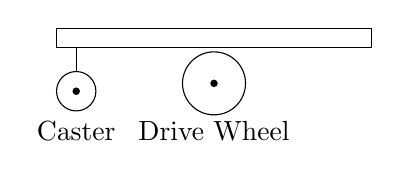
\begin{tikzpicture}
	\begin{scope}[shift={(.25,0)}]
		\node at (0,-.5) {Caster};
		\draw (0,.55) -- (0,0);
		\draw [fill=white](0,0) circle[radius=.25];
		\draw[fill=black] (0,0) circle[radius=.04];
	\end{scope}

	\draw (0,.55) rectangle (4,.8);

	\begin{scope}[shift={(2,0)}]
		\node at (0,-.5) {Drive Wheel};
		\draw (0,.10) circle[radius=.4];
		\draw[fill=black] (0,.10) circle[radius=.04];
	\end{scope}
\end{tikzpicture}

\end{center}
\caption{2 Wheeled Robot (Side view)}
\label{fig:2wheelBot}
\end{figure}

We will begin our analysis with the odometry model of the two wheeled robot. The
odometry model is as follows (its derivation is beyond the scope of this
report):

%TODO make odom graphic
\begin{equation}
\label{eq:deadReckonState}
	P(t) = 
	\begin{bmatrix}
	S \\ \theta
	\end{bmatrix}
	=
	\begin{bmatrix}
	\frac{1}{2}	& \frac{1}{2} \\[0.3em]
	\frac{1}{\mathrm{w}} & -\frac{1}{\mathrm{w}}
	\end{bmatrix} 
	\begin{bmatrix}
	s_R(t) \\ s_L(t)
	\end{bmatrix}
\end{equation}

Where $S$ and $\theta$ respectively are the robot distance travelled and heading
of the robot. $s_L$ and $s_R$ are the distances traveled by each wheel (left and
right respectively). $w$ is the distance between the contact points of the
wheels of the robot.

\begin{figure}[H]
	\begin{center}
	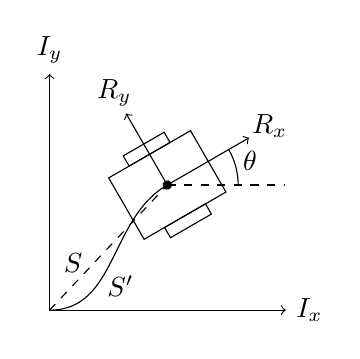
\begin{tikzpicture}[scale=3]
% axis labels
\node at (0,1.1) {$I_y$};
\node at (1.1,0) {$I_x$};

% inertial axis
\draw[<->] (0,1) -- (0,0) -- (1,0);

% robot reference frame
\begin{scope}[rotate around={30:(0.4,0.3)},shift={(0.4,0.3)}]
%wheels 
	\draw (.1,0) rectangle (.3,-0.05);
	\draw (.1,.3) rectangle (.3,.35);
	%robot body
	\draw (0,0) rectangle (0.4,0.3);
	% axis
	\coordinate (C) at (.2,0.15);
	\draw[fill=black] (C) circle [radius=0.05em];
	\draw[<->] (.2,.5) -- (.2,0.15) -- (0.6,0.15);
	% rotation angle
	\begin{scope}[rotate around={-30:(.2,0.15)},shift={(.2,0.15)},dashed]
		\draw[dashed] (0,0) -- (.5,0);
		\draw[solid] (0.3,0) arc [start angle=0,end angle=30, radius=.3];
		\node at (.35,0.1) {$\theta$};
	\end{scope}
	% axis labels
	\node at (.2,.6) {$R_y$};
	\node at (.7,.15) {$R_x$};
\end{scope}
% robot position line
\node at (.1,.2) {$S$};
\draw[-,dashed] (0,0) -- (C);
% robot curve line
\draw (0,0) to [out=0,in=210] (C);
\node at (.3,.1) {$S\mathrm{'}$};
\end{tikzpicture}

	\end{center}
	\caption{Robot Motion Model from $t=0 -$ \delt}
	\label{fig:2wrMotion}
\end{figure}


From \eqref{deadReckonState} we can create a motion model relative to the
inertial frame of reference $I$ (as shown in \figref{2wrMotion}). To simplify
our analysis the following is assumed:

\begin{itemize}
\item The robot's motion model is measured on a time differential \delt that
is small with respect to the total time ($T$) the robot performs its motion. 
\item The robot's wheel encoders are error-less and no wheel slipping occurs.
\item \delt is chosen to be small enough so that $S\mathrm{'}-S \approx 0$ and
thus $S\mathrm{'} = S$.
\end{itemize}

From these assumptions we have a motion model for the robot:

\begin{equation}
\label{eq:motionState}
\xi_{i} = 
\begin{bmatrix}
x \\ y \\ \theta
\end{bmatrix}
=
\begin{bmatrix}
\cos{\theta} & 0\\
\sin{\theta} & 0\\
0 & 1
\end{bmatrix}
P(t_i+\Delta\mathrm{t})-P(t_i)
\end{equation}

$\xi_{i}$ is the position of the robot after some time lapse \delt. Thus to get
the current position of the robot after some time $T$ simply sum the interval
position changes: 

\begin{equation}
\label{eq:sumE}
\xi(T) = \xi_0 + \sum^{n}_{i=0} \xi_{i} : n = \frac{T}{\Delta\mathrm{t}}
\end{equation}

Where $\xi_0$ is the initial position of the robot. 

\eqref{sumE} simply means that given the robots initial position and a sequence
of wheel distance measurements for $t=\{\delT,2\delT,\cdots,T\}$ the position of
the robot at $T$ can be predicted. This of course is only valid for the above
assumptions.

Dead reckoning is not practical when used alone. Sensor noise, wheel slippage,
and distance estimation error ($S-S\mathrm{'}$) all affect the outcome of
\eqref{sumE}.

\subsection{Wheel Encoders}
% usages simple design of quad Encoders sensor readings format (grayscale
% encoding) measuring x/v/a from encoders sources of error

\subsection{Sonar Range Finder}
% usages
% simple design explanation (signal threshold and time of flight)
% error types 

\end{document}
